\documentclass[a4paper,10pt,oneside,final]{article}


\usepackage[english]{babel}
\usepackage[T1]{fontenc}
\usepackage{tabularx}
\usepackage[usenames,dvipsnames]{color}
\usepackage[table]{xcolor}
\usepackage[left=3.0cm, right=2.5cm, top=2.5cm, bottom=2.5cm]{geometry}
\usepackage{graphicx}
\usepackage{float}
\usepackage{caption}
\usepackage{listings}


\lstdefinestyle{ccc} 
{ 
numbers=none, 
basicstyle=\small\ttfamily, 
keywordstyle=\bf\color[rgb]{0,0,0}, 
%commentstyle=\color[rgb]{0.133,0.545,0.133}, 
stringstyle=\color[rgb]{0.627,0.126,0.941}, 
backgroundcolor=\color{white}, 
frame=tb, %frame= lrtb, 
framerule=0.5pt, 
linewidth=\textwidth,
%aboveskip=-4.0pt,
%belowskip=-4.0pt,
lineskip=-5.0pt,
}

%
% Define author(s) and  component's name
%
\def\defauthor{Lasse Lehtonen}
\def\deftitle{FH Ring\\Reference Manual}



\author{\defauthor}
\title{\deftitle}

\usepackage{fancyhdr} 
\pagestyle{fancy} 
\lhead{\bfseries Department of Computer Systems\\
  Faculty of Computing and Electrical Engineering}
\chead{} 
\rhead{\bfseries \deftitle} 
\lfoot{\thepage} 
\cfoot{}
\rfoot{
\includegraphics[height=1.0cm]{pic/tty_logo.png}}
\renewcommand{\headrulewidth}{0.4pt}
\renewcommand{\footrulewidth}{0.4pt}


\def\deftablecolora{blue!10!white}
\def\deftablecolorb{white}

\begin{document}


%\maketitle
%\thispagestyle{empty}

\begin{titlepage}
\begin{center}

\vspace{6.0cm}
\textsc{\LARGE Tampere University of Technology}\\[1.0cm]
\textsc{\Large Faculty of Computing and Electrical Engineering}\\[1.0cm]
\textsc{\Large Department of Computer Systems}\\[1.0cm]
\vspace{6.0cm}
\hrule
\vspace{0.4cm}
{ \huge \bfseries FH Ring\\[0.5cm]Reference Manual}
\vspace{0.4cm}
\hrule

%\vspace{2.0cm}

\vfill

\begin{minipage}{0.4\textwidth}
\begin{flushleft} \large
\emph{Author:}\\
Lasse Lehtonen
\end{flushleft}
\end{minipage}
\begin{minipage}{0.4\textwidth}
\begin{flushright} \large
\emph{Updated:} \\
\today
\end{flushright}
\end{minipage}

\end{center}
\end{titlepage}

\newpage
\tableofcontents



\newpage
\section{REVISION HISTORY}
\setcounter{page}{1}

\begin{center}
  \rowcolors{3}{\deftablecolora}{\deftablecolorb}
  
  \captionof{table}{}
  \begin{tabularx}{\textwidth}{|lllX|}
    \hline
    Revision & Author          & Date       & Description\\
    \hline
    1.00  & Lasse Lehtonen  & 23.8.2011 & Initial documentation\\
    & & & \\
    & & & \\
    & & & \\
    & & & \\
    \hline
  \end{tabularx}
\end{center}



\newpage
\section{DOCUMENT OVERVIEW}

\subsection{SCOPE}

This documentation describes the basic operation and usage of FH Ring
Network-on-Chip component.

\subsection{AUDIENCE}

For hardware integrators wanting to use this component.

\subsection{RELATED DOCUMENTATION}

\begin{center}
  \rowcolors[]{2}{\deftablecolora}{\deftablecolorb}

  \captionof{table}{}
  \begin{tabularx}{\textwidth}{|lX|}
    \hline
    Document & Description\\
    \hline    
    & \\
    & \\
    & \\
    & \\
    \hline
  \end{tabularx}
\end{center}

\subsection{DOCUMENT CONVENTIONS}


\begin{itemize}
\item Ports: \texttt{teletype} in text
\item Generics: \texttt{teletype} in text
\end{itemize}



\newpage
\section{INTRODUCTION}

\subsection{BRIEF DESCRIPTION}

FH Ring Network-on-Chip is a highly configurable network. Network can
be configured to use either store-and-forward of wormhole switching
and has optional diagonal links. Fifo depths and bus widths can be
freely set and the network supports different synchronous frequencies
for agents than the network's operating frequency.

\subsection{EXAMPLE SYSTEM}

Example system in figure~\ref{fig:example_system} presents an eight
agent FH Ring with diagonal links enabled.


\begin{center}  
  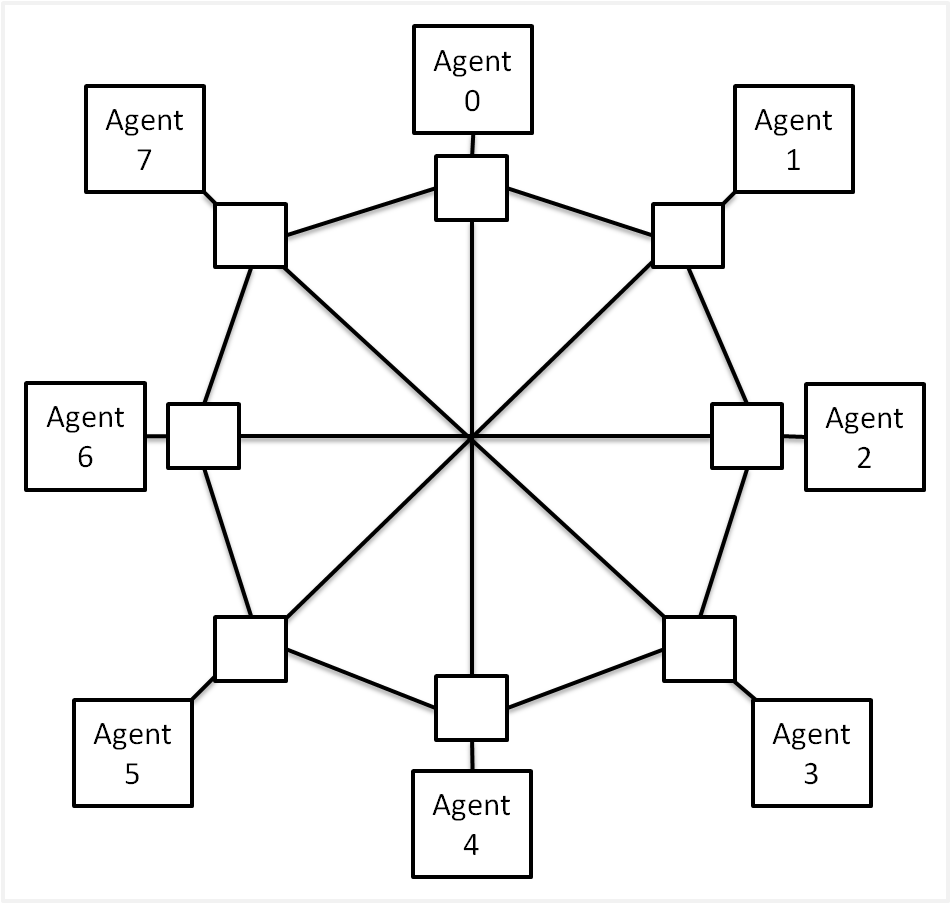
\includegraphics[width=0.8\textwidth]{pic/example_system.png}
  \captionof{figure}{}  
  \label{fig:example_system}
\end{center}



\newpage
\section{HARDWARE DESIGN}

\subsection{FH RING}

\subsubsection{GENERICS}

\begin{center}
  \rowcolors{3}{\deftablecolora}{\deftablecolorb}

  \captionof{table}{}
  \begin{tabularx}{\textwidth}{|lX|}
    \hline
    Name                & Description\\
    \hline
    diag\_en\_g  & Enable diagonal links, requires even amount of agents\\
    n\_ag\_g            & Number of agents NoC connects\\
    stfwd\_en\_g     & Selects between store-and-forward (1) 
                          and wormhole (0) switching\\
    data\_width\_g  & Width of the data bus in bits\\
    addr\_width\_g  & Width of the address bus in bits. Must be less 
                          or equal than data\_width\_g\\
    fifo\_depth\_g   & Depth of FIFOs in words\\
    packet\_length\_g     & Maximum packet size in words\\
    timeout\_g          & How long to wait for packet to fill\\
    lut\_en\_g          & Enable memory mapped address translation\\
    len\_flit\_en\_g  & Enable packet to carry length information in 
                           its own flit\\
    fill\_packet\_g     & Only send full packets\\
    oaddr\_flit\_en\_g  & Enable packet to carry the destination 
                             memory-mapped address\\
    ring\_freq\_g  & Network's frequency relative to IP  frequecy\\
    ip\_freq\_g  & Agent's relative frequency to network frequecy\\
    \hline
  \end{tabularx}
\end{center}

\subsubsection{CLOCKING AND RESET}


\begin{center}
  \rowcolors{3}{\deftablecolora}{\deftablecolorb}

  \captionof{table}{}
  \begin{tabularx}{\textwidth}{|lllX|}
    \hline
    Port   & Width & Direction & Description\\
    \hline
    clk\_net  & 1     & in      & Clock for the network, active on rising edge\\
    clk\_ip   & 1     & in      & Clock for the IP, active on rising edge\\
    rst\_n & 1     & in      & Reset, asynchronous, active low\\
    \hline
  \end{tabularx}
\end{center}

Clock frequencies must be at integer ratio (e.g. 1:3 but not 2:3) and they must
have a synchronized rising edge.

\subsubsection{DATA INTERFACE}

\begin{center}
  \rowcolors{3}{\deftablecolora}{\deftablecolorb}

  \captionof{table}{}
  \begin{tabularx}{\textwidth}{|lllX|}
    \hline
    Port   & Width & Direction & Description\\
    \hline
    tx\_data\_in & n\_ag\_g*data\_width\_g & in  & All TX datas from IPs \\
    tx\_we\_in & n\_ag\_g & in & Write enables from all IPs\\
    tx\_re\_in & n\_ag\_g & in & Read enables from all IPs\\
    rx\_data\_out & n\_ag\_g*data\_width\_g & out & All RX datas from the network\\
    rx\_empty\_out & n\_ag\_g & out &  RX FIFO empty signals\\
    rx\_full\_out & n\_ag\_g & out &  RX FIFO full signals\\
    tx\_empty\_out & n\_ag\_g & out &  TX FIFO empty signals\\
    tx\_full\_out & n\_ag\_g & out &  TX FIFO full signals\\
    \hline
  \end{tabularx}
\end{center}

Routers are connected to vectors starting from 0 and continuing to
$n\_ag\_g-1$.



\subsubsection{ARCHITECTURE}

 Packet Codec is instantiated between the FH Ring and agents to
 enable additional features such as clock domain crossing and address
 translation from memory mapped io addresses to the network address.

\begin{center}  
  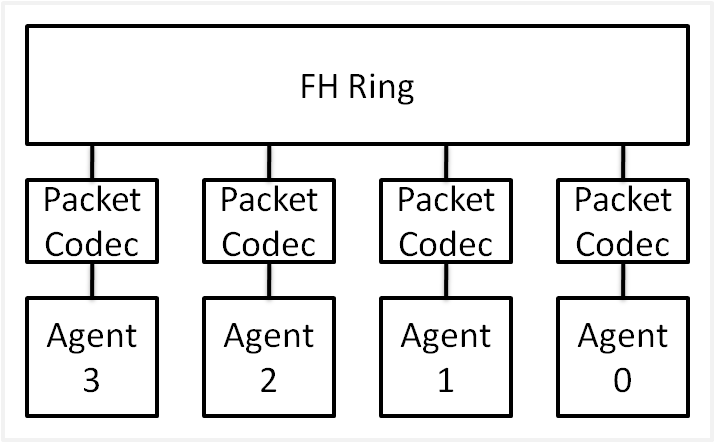
\includegraphics[width=0.4\textwidth]{pic/architecture.png}
  \captionof{figure}{}
\end{center}

\subsubsection{INTEGRATION}

Related  source  files  are listed  in  next  table  in the  order  of
compilation (when applicable).

\begin{center}
  \rowcolors{3}{\deftablecolora}{\deftablecolorb}

  \captionof{table}{}
  \label{tab:files}
  \begin{tabularx}{\textwidth}{|lX|}
    \hline
    Filename   & Description\\
    \hline
    fifo.vhd           & Simple synchronous FIFO\\
    multiclk\_fifo.vhd & FIFO with clock domain crossing\\
    pkt\_counter.vhd   & Debug component counting packets\\   
    addr\_lut\_pkg.vhd & Package for pkt\_codec\\
    addr\_lut.vhd      & Address translation unit\\
    pkt\_enc.vhd       & Packet encoder\\
    pkt\_dec.vhd       & Pakcet decoder\\
    pkt\_enc\_dec\_1d  & Top level for encoders and decoders\\        
    ring\_router.vhd   & Router\\
    ring.vhd           & Top level for FH Ring\\
    ring\_with\_pkt\_codec\_top.vhd & Top level with Packet Codecs\\
    \hline
  \end{tabularx}  
\end{center}


\subsubsection{SWITCHING}

Depending on generic \texttt{stfwd\_en\_g} FH Ring uses either
store-and-forward or wormhole switching. If store-and-forward
switching is used the Packet Codec handles the creation of the network
packet. If there's not enough data to fill the whole packet the unused
flits will be sent empty if \texttt{fill\_packet\_g} is
enabled. Packet Codec will wait few clock cycles before filling the
packet to allow IP to stall a little while sending. For
store-and-forward switching the FIFOs must be the same size as the
packets.

\vspace{0.4cm}
\noindent
For wormhole switched configuration there's no limitation to the size
of the FIFOs.



\newpage
\section{TESTING}

\subsection{TEST CASE}

FH Ring network model comes with a simple test case which instantiates
a six agent ring with packet codec inteface. Test case sends one message
from agent 0 to agent 5 and terminates after that.

\subsection{SIMULATION}

In order to simulate the test case one needs to compile files listed
in table~\ref{tab:files} in addition to files listed in
table~\ref{tab:simfiles} found in basic\_tester/vhd. Top level for the
simulation (simple\_test\_ring.vhd) and the test case files are
located in directory rin/sim. For the users of Modelsim also a
do-file to compile needed files is supplied.


\begin{center}
  \rowcolors{3}{\deftablecolora}{\deftablecolorb}

  \captionof{table}{}
  \label{tab:simfiles}
  \begin{tabularx}{\textwidth}{|lX|}
    \hline
    Filename   & Description\\
    \hline
    txt\_util.vhd          & Helper functions for printing\\
    basic\_tester\_pkg.vhd & Package for Basic Tester\\
    basic\_tester\_tx.vhd  & Transfer generation\\
    basic\_tester\_rx.vhd  & Transfer validator\\
    \hline
  \end{tabularx}  
\end{center}


\end{document}
